% CVPR 2022 Paper Template
% based on the CVPR template provided by Ming-Ming Cheng (https://github.com/MCG-NKU/CVPR_Template)
% modified and extended by Stefan Roth (stefan.roth@NOSPAMtu-darmstadt.de)

\documentclass[10pt,twocolumn,letterpaper]{article}

%%%%%%%%% PAPER TYPE  - PLEASE UPDATE FOR FINAL VERSION
\usepackage[final]{cvpr}      % To produce the REVIEW version
%\usepackage{cvpr}              % To produce the CAMERA-READY version
%\usepackage[pagenumbers]{cvpr} % To force page numbers, e.g. for an arXiv version

% Include other packages here, before hyperref.
\usepackage{graphicx}
\usepackage{amsmath}
\usepackage{amssymb}
\usepackage{booktabs}


% It is strongly recommended to use hyperref, especially for the review version.
% hyperref with option pagebackref eases the reviewers' job.
% Please disable hyperref *only* if you encounter grave issues, e.g. with the
% file validation for the camera-ready version.
%
% If you comment hyperref and then uncomment it, you should delete
% ReviewTempalte.aux before re-running LaTeX.
% (Or just hit 'q' on the first LaTeX run, let it finish, and you
%  should be clear).
\usepackage[pagebackref,breaklinks,colorlinks]{hyperref}
\usepackage[hyphens]{url}


% Support for easy cross-referencing
\usepackage[capitalize]{cleveref}
\crefname{section}{Sec.}{Secs.}
\Crefname{section}{Section}{Sections}
\Crefname{table}{Table}{Tables}
\crefname{table}{Tab.}{Tabs.}

% Custom helpers

\newcounter{refcounter}
\setcounter{refcounter}{1}
\newcommand{\dref}{\label{ref:\arabic{refcounter}}\item[\text{[\arabic{refcounter}]}]\setcounter{refcounter}{\the\numexpr\value{refcounter}+1}}
\newcommand{\rref}[1]{\hyperref[ref:#1]{\text{[#1]}}}
\newcommand{\clickable}[1]{\url{#1}}

\hypersetup{  
    urlcolor=black
}

%%%%%%%%% PAPER ID  - PLEASE UPDATE
\def\cvprPaperID{*****} % *** Enter the CVPR Paper ID here
\def\confName{CVPR}
\def\confYear{2022}


\begin{document}

%%%%%%%%% TITLE - PLEASE UPDATE
\title{Investigating Apples NeuralHash}

\author{Qiankun Zheng, Tim Schneider, Maximilian Löffler\\
Universität des Saarlandes\\
{\tt\small \{qizh00001 / s8tiscne / s8maloef\} @stud.uni-saarland.de}
% For a paper whose authors are all at the same institution,
% omit the following lines up until the closing ``}''.
% Additional authors and addresses can be added with ``\and'',
% just like the second author.
% To save space, use either the email address or home page, not both

}
\maketitle

%%%%%%%%% ABSTRACT
\begin{abstract}
Apple introduced their new strategy of fighting against digital child pornography distribution to the public in August of 2021. The newly proposed strategy, built upon deep hashing technology to detect and report abusive materials, has received a lot of backlashes against users' privacy. In this paper, we investigate the robustness of NeuralHash by using simple image filters to slightly modify the images without changing their contents and discover that $10\%$ to $35\%$ of a hash value can be flipped in our experiments. Furthermore, we train a fully connected neural network to classify these images only based on their hashes and find that neural hashes leak a significant amount of information about the original images' structure and features.
\end{abstract}

%%%%%%%%% BODY TEXT

\section{Introduction}
\label{sec:intro}
Child sexual abuse material (CSAM) is no new problem. For years now it left a trace of frustration in many governments and companies and has been used to argue for several privacy critical decisions. As there has been a siginificant increase in reported CSAM material with each new year \rref{4} the pressure is building up on big technology companies to assist in CSAM detection and prevention, and towards the end of last year Apple decided to reveal their take on this problematic.  

Fundamentally it relies on a neural network to produce a fingerprint for a file being uploaded to iCloud. Those fingerprints will be checked against a database of known fingerprints of CSAM and upon a big enough reassemblence the file will flagged. After a threshold of thirty flagged images Apple can take action and manually investigate the users cloud system.

Despite emphasizing their privacy focused approach the feature was not perceived well. After a quick wave of criticism from the digital privacy community \rref{5} Apple decided to delay working on it to reevaluate data privacy and abusability of the system for an unspecified time. Nonetheless we can expect the feature to arrive in this or a similar format sooner or later. 

The problems with Apples idea many privacy researchers and activists pointed out are various. If neural-hashes preserve properties of the original footage then someone with access to the hashes of a victim might be able to reconstruct their images.Furthermore if adversaries are able to produce images with arbitrary neural-hashes then they could continue their illegal businesses and most critically: with a little insight to the``secret database'' of CSAM hashes they could produce benign images with malicious hashes to either DoS Apple by producing infinitely many CSAM warnings, effectively rendering the system useless, or distribute the tempered files to known activists or journalists which gives then Apple a reasons to access their files for manual review. This attack could therefore also be misused by malicious governments in cooperation with Apple to spy on critical subjects \rref{6}.

Taking this into account it is of obvious public interest that such a feature is being implemented in a way which is not succeptable to the previously mentioned attacks. In the following we probe Apples NeuralHash under two aspects:

\begin{enumerate}

\item \textbf{Reclassification}: We train a separate model to reassign labels to neural-hashes to see if hashes preserve information. A secure hashing function would not be reversable.

\item \textbf{Detection evasion}: We apply regular image filtering methods and observe the amount of change in the resulting hash. If a filter exists that changes the hash significantly then criminals have an easy way of hiding CSAM.

\end{enumerate}

\section{Background}
\label{sec:background}

Before we go into detail on the attacks we first want to formalize the notion of ``neural hashing'' which is the foundation of the NeuralHash algorithm. Essentially neural hashing relies on two separate components. \textit{First} a neural network which extracts features from the input image and outputs a $n$-dimensional vector. \textit{Second} a locality sensitive hashing algorithm which assigns the vector a hash value based on its direction in the $n$-dimensional space \rref{3}.

\textbf{Preprocessing}. First we need to transform the input to fit the shape of our network. The preprocessing step in NeuralHash does just this: $pre(inp): (W \times H \times 3) \rightarrow (360 \times 360 \times 3)$.

\textbf{Extracting Features}. Here we insert the prepared input into the network $N(prep) : (360 \times 360 \times 3) \rightarrow (1 \times 128)$ which extracts the most significant image features.

\textbf{Locality sensitive hashing}. The $LSH(vec) : (1 \times 128) \rightarrow (1 \times 96)$ algorithm splits the vector room by inserting $96$ hyperplanes. If a vector point lies on one side of plane $p_t$ assign output bit $b_t$ with $1$ else assign it with $0$.

\textbf{All together}. Now we can define neural hashing as follows $h(inp) = hex(LSH(N(pre(inp))))$. 

\section{Reclassification}
\label{sec:reclass}

One core feature of NeuralHash is that similar images receive similar hash values. We can therefore assume that the underlying network is to a certain degree encoding image features in the hashes which we might be able to extract again. A potential attacker with access to the victims hashes might be able to reobtain the corresponding files and leak information.

\subsection{Experimental setup}

There is no widely known source for labeled neural-hashes yet so we needed to contsruct our own dataset. We selected nineteen of the most populated categories from the core OpenImages dataset, which is maintained by Google, and extracted 1000 samples each to calculated the neural-hashes. 

Then we fed the hashes into our network. For the model we used a fully connected neural network with three hidden layers and ReLU activation functions. We used negative log likelihood as a loss function and SGD optimization. 

\subsection{Results}

We present our results in \hyperref[tab:one]{Table 1}. We observe that our network was able to correctly classify some hashes. The probability for random guessing is around $5.2\%$ so for all but two categories our network could succeeded. This variance is most likely based on the small sample space we had.  We can also observe that classes reassembling humans generally performed worse. We assume this is because it is more likely to missclassify a man for a woman, or even a person then missclassifying a building for a tree. 

\begin{table}
  \centering
  \begin{tabular}{@{}lc@{}}
    \toprule
    \textbf{Class} & \textbf{Accuracy} \\
    \midrule
    Tree & $21.0\%$ \\
    Plant & $15.5\%$ \\
    Building & $13.0\%$ \\
    Human Hair & $12.5\%$ \\
    Footwear & $9.5\%$ \\
    Table & $8.5\%$ \\
    House & $8.0\%$ \\
    \bottomrule
  \end{tabular}
  \hspace{10px}
  \begin{tabular}{@{}lc@{}}
    \toprule
    \textbf{Class} & \textbf{Accuracy} \\
    \midrule
    Man & $8.0\%$ \\
    Glasses & $7.5\%$ \\
    Car & $7.0\%$ \\
    Woman & $6.5\%$ \\
    Girl & $6.5\%$ \\
    Person & $5.0\%$ \\
    Boy & $1.0\%$ \\
    \bottomrule
  \end{tabular}
  \caption{Classification accuracy of our model. Find the image category the left column and how often hashes of images of this category have been correctly assigned to this category.}
  \label{tab:one}
\end{table}

This assumption is vagely backed up by our \textit{Top-X-Classification} results summarized in \hyperref[tab:two]{Table 2}. We succeed in categorizing our labels to groups of $3$ with probability $24.1\%$, here we assume that grouping categories would introduce supercategories for pictures of humans or nature. This clustering results from our choice of overlapping label classes, for example a picture of a young woman can also be a picture of an old girl and contain human hair or a dress. This clustering is displayed in \hyperref[tab:three]{Table 3}.

\begin{table}
  \centering
  \begin{tabular}{@{}ccc@{}}
    \toprule
    \textbf{Top-1} & \textbf{Top-3} & \textbf{Top-5} \\
    \midrule
    $9.2\%$ & $24.1\%$ & $37.0\%$  \\
    \bottomrule
  \end{tabular}
  \caption{Combined top accuracies over all labels. Values indicate that categorization task is feasible for our network.}
  \label{tab:two}
\end{table}

\begin{table}
  \centering
  \begin{tabular}{@{}c|ccc@{}}
    \toprule
    \textbf{Label} & \textbf{Top guess} & \textbf{Second} & \textbf{Third} \\
    \midrule
     Car & Car ($14$) & Window ($11$) & Plant ($10$) \\
     Woman & Girl ($11$) & Human Hair ($9$) & Dress ($8$) \\
     Window & Window ($14$) & Building ($12$) & Plant ($11$) \\
    \bottomrule
  \end{tabular}
  \caption{Selection of labels and respectively most assigned outputs by our network. Entries under Label represent the original label, values under Top guess, Second and Third represent the values which have been assigned most throughout 100 test runs with according percentage. Example: In $11\%$ of queries to our network a hash of a Woman picture was classified as Girl.}
  \label{tab:three}
\end{table}

In summary we can validate our initial assumption that neural hashes preserve information about the corresponding images. A more suffisticatledy trained network might be able to \textit{firstly} classify and categorize with siginificantly higher probability \rref{2} and \textit{secondly} attempt to recreate certain image features from just the hash. 

\section{Detection Evasion}
\label{sec:detec_evad}

There are two different approaches to evade detection under NeuralHash, the first being gradient-based. As the hashing of images has to be done locally to ensure user privacy, Apple has to ship their model with each device making a white-box adversarial attack like FGSM feasible. The second attacking vector is applying basic image manipulation. 

While the first approach promises a very high accuracy and low pertubation it might be the more unrealistic attacking scenario under the assumption that a majority of CSAM distributors do not know how to perform such an attack. In the following we mainly discuss the latter threat model. 

\subsection{Experimental setup}

We again use the OpenImages dataset, considering the original attacking scenario of CSAM detection we focused on images of persons.  We made use of 500 individual samples on which we applied three basic image filtering strategies: sepia, contrast and a mixture of sepia, contrast and vibrance. All filters were taken from the python library FImage. The choice of filters is based on accessibility, we want simple filters which every attacking person can make use of. This mimics a realistic mediocrely technology savvy adversary.

After applying the filters we measured the difference between the original neural-hash and the tempered one in bits. We calculated the average bit-flipping rate over the dataset to get a better estimation.

\subsection{Results}

\subsubsection{Manipulation weights}

The sepia filter mostly changes the saturation of the image. This transformation can be observed to produce the least amount of bitflips in general with $4.91\%$ on $50\%$ filter strenght and $13.54\%$ on $100\%$. The sepia filter produces the least distorted image, samples are displayed in \hyperref[fig:three]{Figure 3}.

The contrast filter achieves $26.61\%$ and $32.94\%$ bitflips respectively while creating a result which appears more disturbed to the human eye then sepia. Nonetheless this flip rate is quite significant. The filter relies on exaggerating the difference in brighter and darker sections.  

The mix filter achieves similar results to contrast. While images with applies filters are by no mean non-transformed they can be very clearly recognized by the human eye.  

\begin{figure}[t]
  \centering
  \fbox{\rule{0pt}{0.5in} 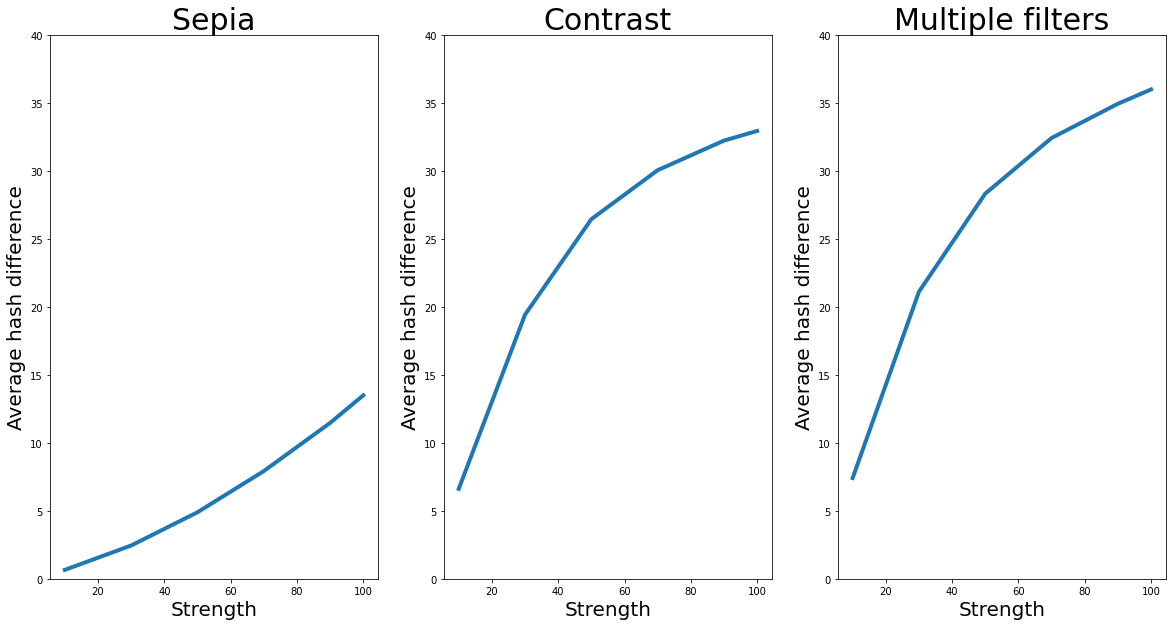
\includegraphics[width=0.8\linewidth]{bitflips1}\rule{0.03\linewidth}{0pt}}
   \caption{Average bitflips on dataset of persons for sepia, contrast and mix filter respectively. }
   \label{fig:one}
\end{figure}

\begin{figure}[t]
  \centering
  \fbox{\rule{0pt}{0.5in} 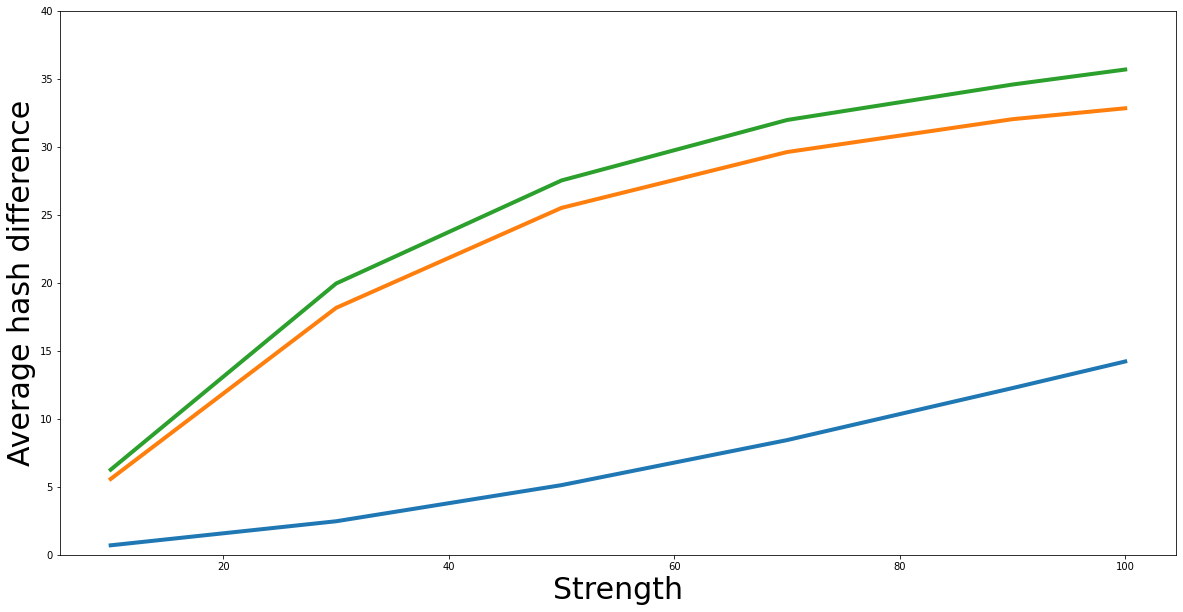
\includegraphics[width=0.8\linewidth]{bitflips2}\rule{0.03\linewidth}{0pt}}
   \caption{Average bitflips on dataset of buildings for sepia (blue), contrast (orange) and mix filter (green). The results match up with the those of the persons dataset.}
   \label{fig:two}
\end{figure}

\subsubsection{Generalization}

To find out if the model has specifically been trained on images of humans we repeat the experiments on different datasets of non-human subjects. In summary the results can be seen when comparing \hyperref[fig:two]{Figure 2} with \hyperref[fig:one]{Figure 1}. There is no major difference in results indicating that the model was not specifically trained on human samples. It is up to further research whether models specifically trained on humans can be more resilient to detection evasion attacks on CSAM.

\begin{figure}[t]
  \centering
  \fbox{\rule{0pt}{0.5in} 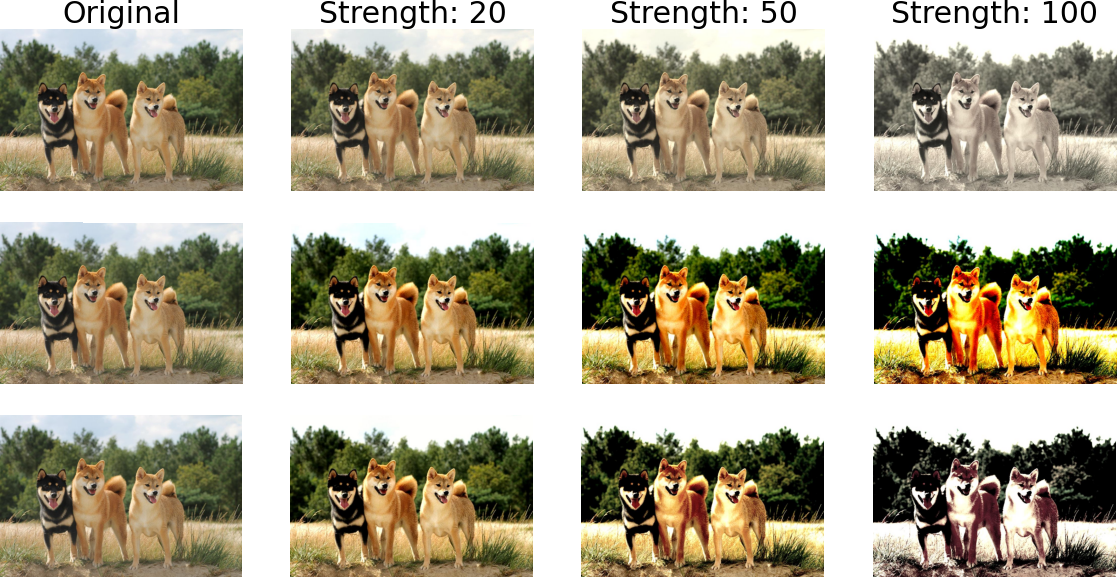
\includegraphics[width=0.8\linewidth]{example_images}
  \rule{0.0\linewidth}{0pt}}
   \caption{Demonstration of filters with increasing strenght. First row sepia, second contrast, last row mixed filters.}
   \label{fig:three}
\end{figure}

\subsubsection{Countermeasures}

The robustness of NeuralHash is questionable, it can be fooled with filters natively available on every Apple device. Research by Struppek et. al \rref{2} has shown that image transformations like croping, rotating or mirroring can cause similar effects and gradient based attacks nearly achieve $100\%$ detection evasion with little pertubations applied. 

It is reasonable to assume that Apple already trained the model on ``adversarial'' images as the models purpose is to classify slightly manipulated images with the same hash value. Similar hardening techniques will likely not increase robustness. 

One possible defense is increasing the hash length \rref{1} as this allowes the model to encode more features of the footage into the hash. While this would likely help robustness it would also easen the Reclassification attack described in \hyperref[sec:reclass]{Section 3}.

\section{Conclusion}

While the intentions behind NeuralHash for CSAM detections are good this technology undermines user privacy and opens the gates for systematic discrimination while knowledgable attackers can bypass the system all together without a problem. It is important that the research community further investigates this subject. Open questions include: Is it possible to recreate entire images from neural hashes? Can detection evasion be realistically prevented with elongated hashes? Do more efficient detection evasion techniques exist? If the trust in technology is broken once restoring it will be nearly impossible.

\section{References}

\begin{itemize}
	
	\dref Jain S., Cretu A.M., and de Montjoye Y.A. ``Adversarial Detection Avoidance Attacks: Evaluating the robustness of perceptual hashing-based client-side scanning''.  2021, USENIX.
	
	\dref Struppek L., Hintersdorf D., Neider D. and Kersting K.  ``Learning to Break Deep Perceptual Hashing: The Use Case NeuralHash'', 2021, arXiv:2111.06628v2.
	
	\dref \clickable{https://www.apple.com/child-safety/pdf/
	CSAM\_Detection\_Technical\_Summary.pdf} Aug 2021, Technical documentation of NeuralHash.
	
	\dref \clickable{https://www.missingkids.org/content/ncmec/en/blog/2021/rise-in-online-enticement-and-other-trends--ncmec-releases-2020-.html} 24 Feb 2021, Report on CSAM amount by NCMEC.
	
	\dref \clickable{https://edwardsnowden.substack.com/p/all-seeing-i}, 26 Aug 2021, Edward Snowden discussing implications of CSAM detection on Apple devices.
	
	\dref \clickable{https://www.nytimes.com/2021/10/14/business/apple-child-sex-abuse-cybersecurity.html}, 14 Oct 2021, New York Times summing up experts concern about iCloud scanning techniques. 
	
\end{itemize}

 

%%%%%%%%% REFERENCES
{\small
\bibliographystyle{ieee_fullname}
\bibliography{egbib}
}

\end{document}
